\chapter{Phase 3 --- Improving the UI/UX}
Phase 3 was the first of the two shorter phases focusing on UI iteration. It spanned approximately two weeks, starting with the implementation of the new UI, and ending with the second of the three focus groups with first year undergraduate students. 

\section{Requirements Analysis}
The motivations for this phase come mainly from the advanced focus group, however requirements from the \hyperref[sec:c1_autoethnography]{autoethnographic phase} of the project, as well as the \hyperref[eval:c1]{proof of concept client meeting} continue to be relevant. 

The advanced focus group was generally very positive about the language, but they had many thoughts about the Proof of Concept UI they were presented with. During phase 2, I created a Figma prototype for the next UI (see \ref{c2:next_ui}). Many of their thoughts about the Proof of Concept UI were things that were already addressed with the new design. This prototype was presented to the advanced focus group, who much preferred it. The advanced focus group had no criticism of the new UI, so it should be implemented as designed for now. 

The prototype for the new UI also included the functionality to `undo progress', by clicking on a previous program state in the table to make this the current version of the program. The advanced focus group appreciated this functionality. 

% \section{Design}
% Because I wanted to be able to evaluate the prototype for the web UI with the advanced focus group, the web UI was designed in the last phase. I set aside time to design 


% \todo{there was no design here? the advanced focus group liked the protype a lot and did not have any }

\section{Implementation}
Implementing the new UI mostly consisted of time-consuming React and CSS tweaks which are not worth mentioning here. However, there were some more challenging aspects that required some more interesting considerations and changes to be made. Screenshots of the result of implementing the new UI with these features is shown in \ref{screenshot:phase3_end_lazy}, with another example showing free choice evaluation in the appendix \ref{screenshot:phase3_end_free}. 


\subsubsection{Diff}
\label{paragraph:diff} 
Our frontend requires the ability to see what has changed between two program states. Highlighting these changes make understanding the changes in the users program in the frontend easier. This function generates the strings for the two trees simultaneously, producing the similarities and differences. If two nodes are different structures, then we turn them into strings and regard them as differences. However, if two nodes are the same structure, we identify what parts of that structure are similarities and what parts are differences. For instance, if the algorithm is called on an application, we generate the diff for the function and for the argument separately, and then concatenate the diffs. \ref{fig:diff_list} shows a subsection of this algorithm, showing how it works for IDs, Literals and Pairs. 

% Move to c4
% \subsubsection{Syntax Highlighting}
% \subsubsection{Display RC history}
% We also wish to         

\subsubsection{Reduction Messages}
Rather than presenting the user with simply the before and after of the reduction, this design calls for presenting the user with a message describing what will happen. While generating the options for reduction (see \ref{c1_design_reduction_progress}), we can keep track of information relevant to how it was generated to inform the message displayed. For instance, if a reduction is generated from the application of a named function with name A to two arguments B, C, we can convert those arguments to strings and then broadcast the message `Applied function A to B and C'. 

If B or C are large pieces of syntax, this may generate a very large unintelligible string. To solve this, we can modify our stringification algorithm to do certain things different to normal:
\begin{itemize}
    \item Do not show the cases of a match statement, as the condition should be enough differentiate it
    \item We can truncate the output to a fixed length 
\end{itemize}

In past iterations, redex-contraction pairs were passed to the front end as two strings. We can make it three strings instead, where one of the strings is the reduction message which can be displayed before the reduction. The other two strings, the redex and contraction, can be displayed after the reduction in the history. 

\subsubsection{Revert Progress Functionality}
We may wish to undo progress. This was functionality designed into the new UI that the advanced focus group specifically mentioned liking. 

Undoing progress requires that previous \ac{AST} states must be stored. Before now, the most recent \ac{AST} state was stored at a known memory address so any of the functions in the binary could know where to find it. This was done to avoid having to pass the \ac{AST} to the JavaScript module. If we wanted to store the history of all \ac{AST}s, one approach could be to store all the \ac{AST}s in a pre-allocated memory region in a stack, and then allow the JavaScript module to refer to each of the \ac{AST}s in the history by their stack index. However, pre-allocating enough memory for any potential program execution logs would be misguided, as it would cause accessibility problems for computers with less memory. Instead, we should employ dynamic allocation. 

The issue with dynamic allocation of memory for the \ac{AST}s as they are added to our history is that we no longer know exactly where they will be located, meaning this information must be stored such that it will not be erased between calls to \ac{WASM} library functions. One method of doing this is passing a pointer to where in memory the \ac{AST} is located to the JavaScript module so that it can refer to it later, and use library functions on it. At first glance, this sounds like a bad idea, as when pointers are returned from a function for which wasm-bindgen (see~\ref{bg:wasm-bindgen}) is used to make a JavaScript binding, the pointer is represented as a JavaScript $number$ type~\cite{wasm_bindgen_guide}, which is a double-precision IEEE-754 value~\cite{ecma262number}. Storing pointers as floating point values, and then attempting to dereference them, sounds like a recipe for memory mismanagement. However, this is safe because WebAssembly 2.0 has 32 (see~\ref{bg:wasm}), and thus has 32 bit pointers, and a double precision floating point number has a 52 bit~\cite{ieee754} mantissa meaning it can safely store the 32-bit memory location without issue. 

In our JavaScript module, we can then store a stack of pointers to the \ac{AST}s, and display the options for reducing the one at the top. When an option is selected, we can apply the reduction and then store the new \ac{AST} on the top of our stack and recalculate reduction options. If the user decides to start evaluating a new program, all the \ac{AST}s with pointers in this list are freed to avoid memory leaks.

\begin{figure}[h]
    \centering
    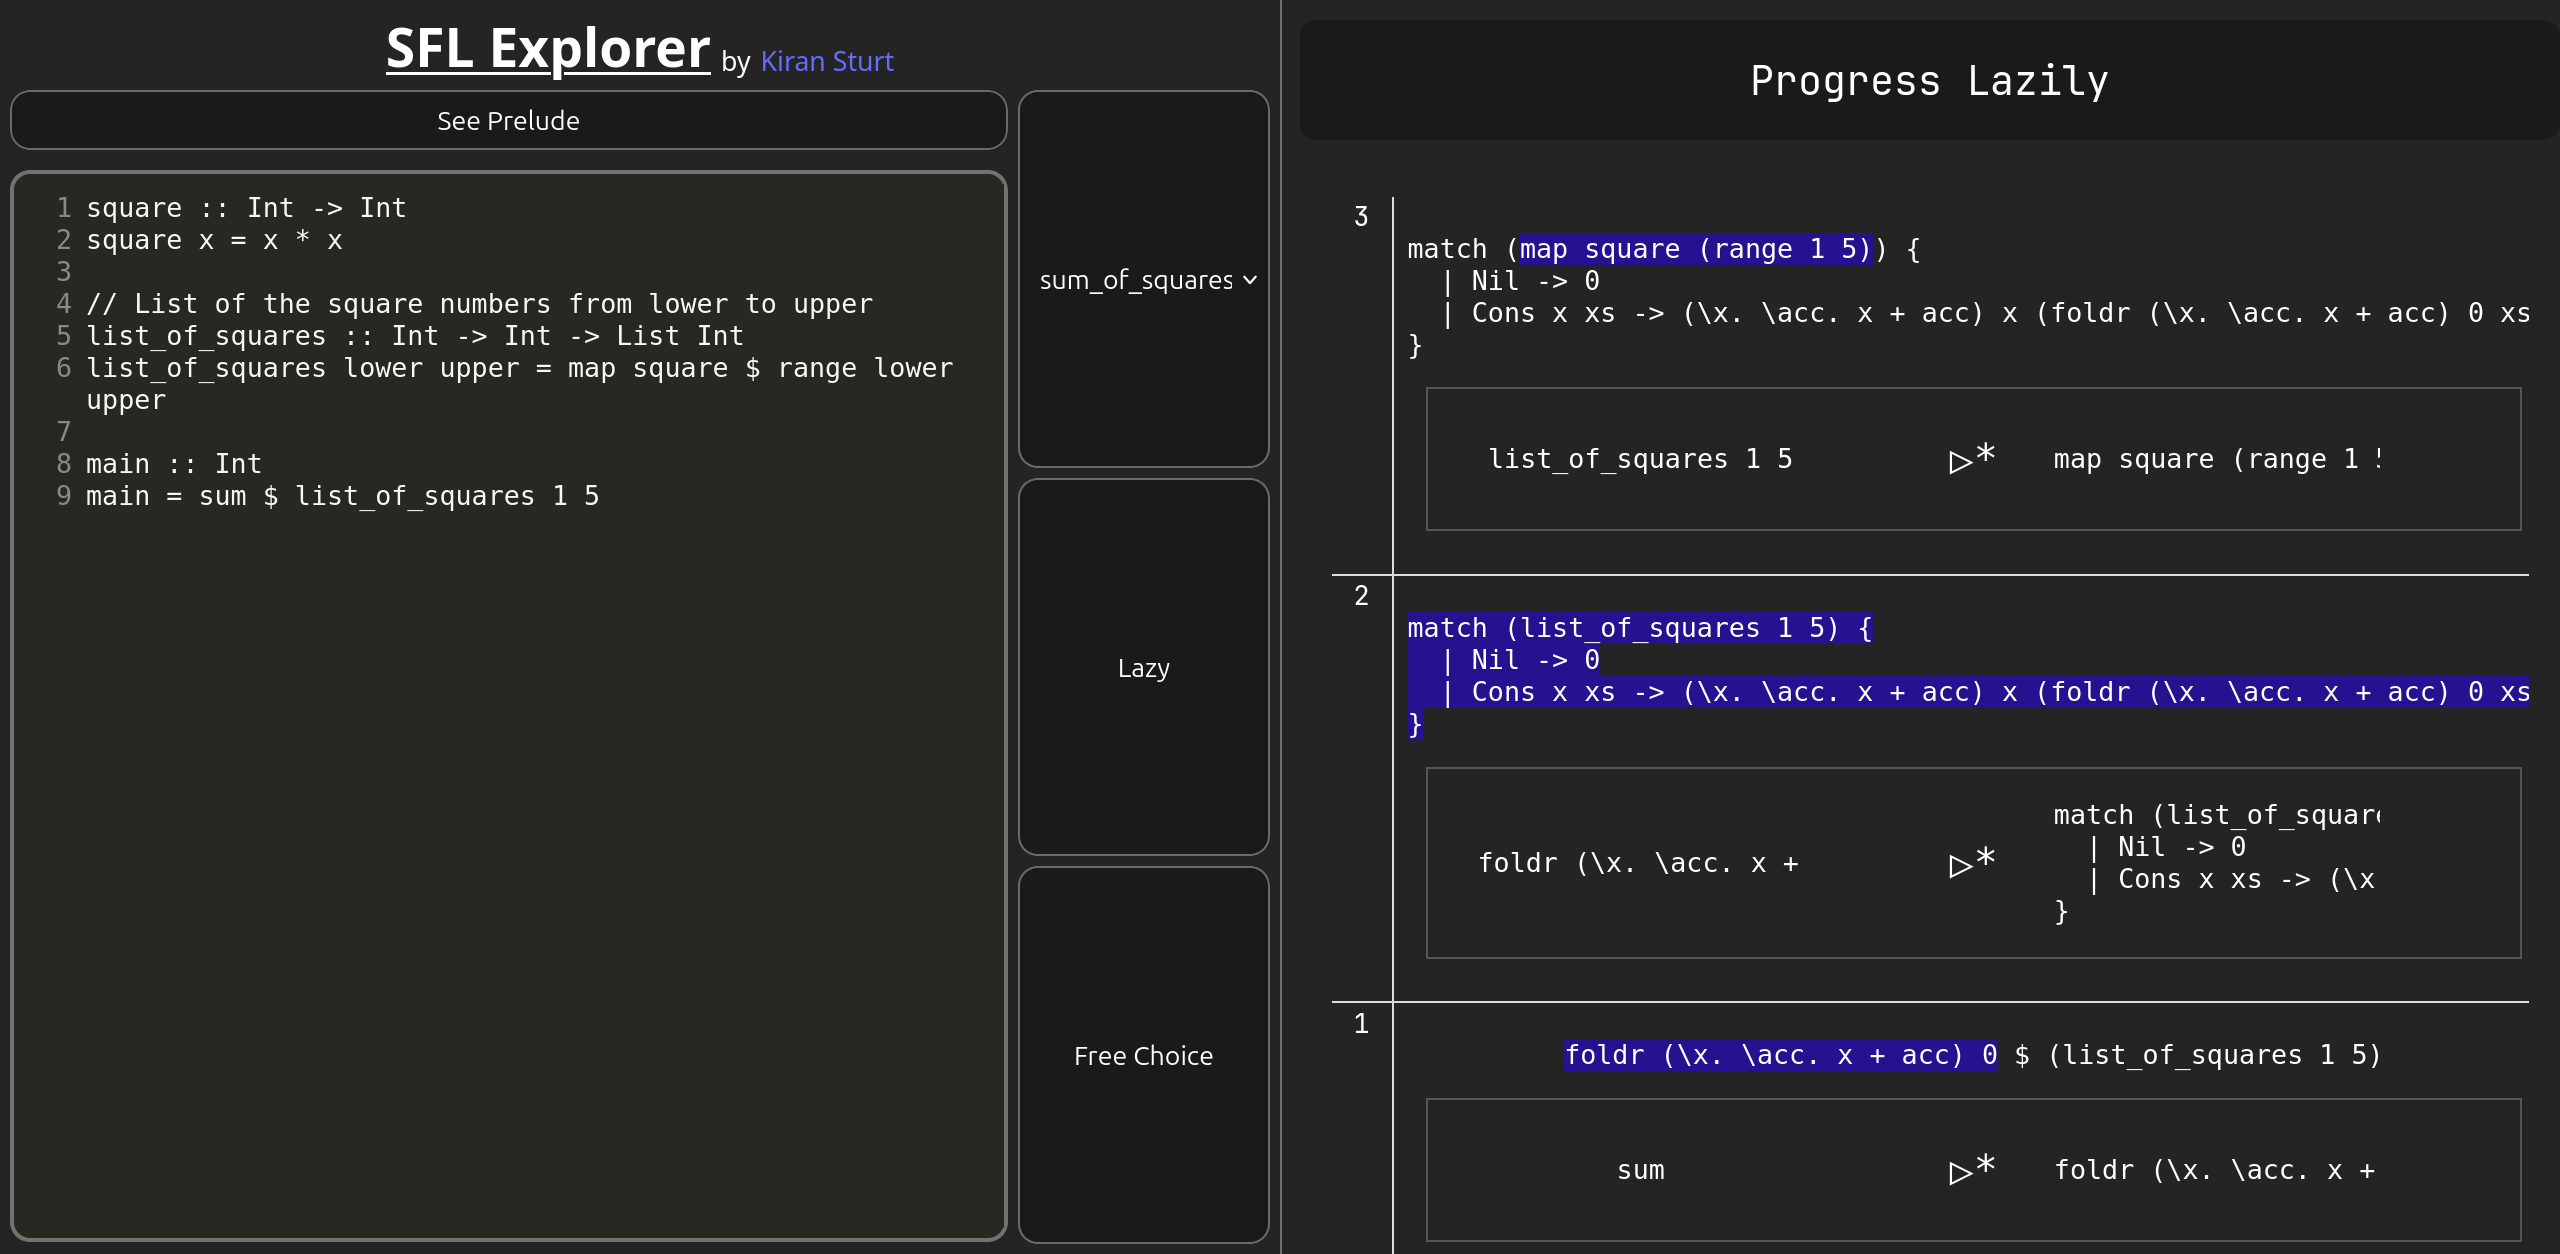
\includegraphics[width=\linewidth]{images/phase-3-end.png}
    \caption{The new UI implemented, during lazy evaluation of the provided `sum of squares' example program}
    \label{screenshot:phase3_end_lazy}
\end{figure}

\section{The Intermediate Focus Group: Evaluation and Next Steps}
\label{eval:IFG}
The Intermediate focus group happened at the end of phase 3 of the project. An entirely different structure was employed for this focus group than the Advanced Focus Group \ref{ref:afg}, as the aims of this focus group were different. Rather than just evaluating the language, I wanted to evaluate the system in the setting that I expected it to be used in: a lecture setting. 

To act as a lecturer, I employed Amos Holland, a fourth year undergraduate student. I considered doing it myself, but I decided that it would be better to employ an undergraduate who was more experienced in teaching functional programming. Amos was selected as he had taken all of the functional programming units that were available in his degree so far: the same ones that the participants of the Advanced Focus Group had taken (for details of these units, see \ref{ref:afg}). Furthermore, Amos had acted as a teaching assistant on two of these units, Types and Lambda Calculus, where he ran weekly problem classes, where he would walk students through difficult problems from the lectures or worksheets, and \hyperref[COMS10016]{COMS10016} where he had been a teaching assignment working in labs in the same capacity as I had. 

\subsection{Selection and Format}
For this focus, to evaluate SFL explorer as a teaching tool and get feedback, I selected first year undergraduate students who had just taken the functional programming unit. I looked for people who had not explored functional programming outside this unit, and who found the unit difficult, as these are representative of group of people the tool would be most useful for. 

\subsection{Bugs}
There were numerous bugs that Amos and I identified during the lecture phase of this focus group:
\begin{itemize}
    \item The editor would sometimes add tab spaces randomly.
    \item Sometimes, the site would refresh on its own.
    \item The editor did not save input consistently.
\end{itemize}
\noindent These were all fixed as part of phase 4.

\subsection{Outcomes}
Due to technical issues, I was only able to get a transcript of the interview portion of the intermediate focus group; I made the mistake of holding this focus group in a room where there was too much background noise to get a high quality recording during this part of the session. However, during the interview, I set up multiple microphones, and was able to combine the AI transcripts from each of them into one transcript. The transcript is in the additional materials \ref{appx:additional_mats}. 

Below is the summary of outcomes from the discussion with this focus group, along with timestamped quotes where relevant. The first phase of this interview was conducted with Amos, followed by an interview with each participant in turn. 

All four participants, and Amos, liked SFL explorer as a whole. 
\noindent\begin{quotation}
\noindent`I think it was good, other than the few bugs' [Amos, 00:04]
\end{quotation}
\noindent\begin{quotation}
\noindent`Yeah, I liked it; this is what I do in my head basically when I'm looking at Haskell, it [the lecture using the tool] was good' [Participant 1, 06:44]
\end{quotation}
\noindent\begin{quotation}
\noindent`I really like what the tool does, like it
shows like what you can see because that's basically what I do when I'm like debugging code but
um it takes like a long time to do it like by hand and to go through everything and sometimes it's
like wrong if you do it yourself so this is like a good way to automate it' [Participant 2, 15:20]
\end{quotation}
\noindent\begin{quotation}
\noindent`I liked it' [Participant 3, 19:07]
\end{quotation}
\noindent\begin{quotation}
\noindent`I actually really love the functionality of this app' [Participant 4, 24:44]
\end{quotation}


In the Advanced Focus Group outcomes section \ref{ref:afg}, I split the focus group's thoughts into positives and negatives. However, in this focus group opinions were more split between participants, as well as participants being more frequently in two minds, so I did not do this. Instead, I have grouped by topic rather than by positivity and negativity, so one bullet point may have both positive and negative thoughts towards the same issue. 

\subsubsection{The Language}
Below is the summary of Amos's and the participants' thoughts about \ac{SFL}, along with timestamped quotes where appropriate.
\paragraph{Amos}
\begin{itemize}

    \item Amos liked the explicit match statement:
    
    `I quite like match, because I think it gets a bit more directly at what pattern matching is doing, like that it's a specific operation' [03:36]

    \item Amos was happy with the language and its features
    
    `There are features of Haskell it doesn't have, but Haskell is a very advanced language. For teaching functional programming, I think it's got the right range of features' [Amos, 00:04]

    \item Amos identified adding type classes as a potential next step 
    
    `If you were to take this, like, a step further, make it more advanced, I think the next step is type
    classes' [Amos, 00:04]
    
    \item `I like the stuff we put in the prelude because we have like sort of basic functions' [Amos, 00:04]
    
    
\end{itemize}

\paragraph{The Participants}\begin{itemize}
    \item They had mixed opinions on whether I should add the usual syntax sugar for lists. Below are two quotes from two participants, showing their split minds on this topic:
    
    `I both love and hate the list, the lack of syntactic sugar for list, \ldots it makes literal lists really hard to read, but it makes the types so much clearer. Having to interact with that rather than just going, that's kind of an array \ldots It really explicitly forces you to think in the Haskell
    way' [Participant 1, 14:47]
    
    `I really liked that, like, well, because we don't have the constructor we had in Haskell
    for, like, lists. Abundantly much clearer to me what was going on \ldots I prefer it with this list, this cons and the nil. But also you have to write it out for five hours as the teacher' [Participant 3, 22:52]

    \item They liked the explicit match statements. 
    
    `I honestly really liked the match being, like, write match. Yeah. So the
    explicitness was good. I really liked that. It made it obvious to me in a way that it wasn't necessarily before \ldots\ This is much easier to learn about pattern matching with than Haskell' [Participant 3, 19:07]
\end{itemize}

\subsubsection{The User Interface, and the System as a Whole}
An absolutely critical issue that became obvious during the focus group was the need for a light mode. The room was very bright, and it was barely visible in dark mode. This was resolved with a high priority in the next phase. 
Below a more detailed summary of their thoughts about SFL Explorer as a whole, and the UI/UX:

\paragraph{Amos}\begin{itemize}
    \item Amos was generally happy with the UI for teaching.
    
    `As far as the design went, I think I was happy with it for teaching' [Amos, 00:04]
    \item A `step to the end' options would be good, allowing the user to complete evaluation without having to click on the button many times.
    
    `It would have been nice to have a button that says steps to the end, because there were some cases where I would have liked to just see if it evaluated correctly, but
    instead you had to click through a lot of times' [Amos, 00:04]
    \item Amos wanted to be able to save more programs than just one.
    
    `It would be nice to be able to define more complete programs and save them so that you can jump between them a bit' [Amos, 02:57]
\end{itemize}

\paragraph{The Participants}\begin{itemize}
    \item They wanted syntax highlighting, indeed 3 out of four explicitly asked for it. 

    \item Two of the participants agreed that the history should be shown in reverse, so it would generate top down, the other two did not comment. 
    \item One participant specifically mentioned liking the way the UI separates the editor from the output
    
    `I like that it's separate. Text editor here. Then this bit shows what it does' [18:02]
    \item They liked how it highlights what has changed between iterations:
    
    `I really like the highlighting in like what changed' [Participant 2, 15:20]
    
    `I, like, as a minor visual thing, \dots\ like, you have the blue bit of the bit you've changed on the right-hand side' [Participant 3, 19:07]
\end{itemize}


\section{Phase 3 Conclusion}
This phase resulted in a high quality UI that was much more polished than the previous iteration. The UI was generally popular with the focus group, and the language continued to be well liked. However, there were many ideas for improvements to be made, the clearest one being adding a light mode. 

% The aims of this focus group were to use the system and attempt to recap functional programming concepts 

% Evaluation:
% - They liked explicit match: they liked it more than haskell for learning about how pattern matching works
% - Really Really needed light mode
% - Horizontal overflow bug